\section{Direkte Fernlokalisierung mit IEEE 802.11}
\label{ch:phase2}
Bei der direkten Fernlokalisierung wird die Messgröße auf den Basisstationen gemessen.
Die Ortungsinformation wird dann implizit durch versenden der gemessenen Werte an den Ortungsdienst übermittelt.
Dieser berechnet dann aus den gesammelten Werten die Position der mobilen Einheit.
Eine Lösung zur direkten Fernlokalisierung muss deshalb nicht mit einem \emph{Access Point} assoziiert sein.
APs versenden die gemessenen Werte jedoch nicht automatisch an den Ortungsdienst. 
Sollen also die APs des WLAN-Netzwerks auch als Basisstationen verwendet werden, muss ihre Software es erlauben den in der Analyse als Messgröße ausgewählten \emph{Received Signal Strength Indicator} (RSSI) bestimmter Pakete abzurufen.

%TODO Tags weg
\subsection{RADAR-Implementierung}
Eine mobile Einheit mit \emph{RADAR} versendet alle 0,25 Sekunden ein 6 Byte langes UDP-Paket, der RSSI der Übertragung wird dann auf dem AP gemessen.
Das Sendeintervall wurde so kurz gewählt, um spontane Schwankungen im RSSI durch mehrfache Messung zu glätten und sich bewegende Personen möglichst genau zu erfassen.
Für eine Bereichsortung reicht ein wesentlich längeres Sendeintervall, es wird erneut ein Intervall von fünf Sekunden gewählt, in dem sich ein Mitarbeiter maximal 42 Meter bewegt. 
Tabelle \ref{table:radarconsumption} zeigt den mit dem \emph{TM103} gemessenen Verbrauch der Implementierung für mobile Einheiten mit \emph{RADAR} jeweils in Arduino und C, mit unterschiedlich langen Sendeintervallen mit und ohne manuellen \texttt{light\_sleep}.

\begin{table}[h]
	\centering
	\caption{Stromverbrauch RADAR-artiger mobiler Einheiten}
	\label{table:radarconsumption}
	\begin{tabular}{l|p{2.2cm}|R{1.5cm}|R{2cm}|R{2cm}|R{2cm}}
		SDK & manueller \texttt{light\_sleep} & Sende"-intervall in s & Versuchs-dauer in Stunden & Gesamt-verbrauch in mAh & $\varnothing$ Verbrauch in mA \\
		\hline
		Arduino Core & Nein & 0,25 & 2 & 80 & 40,00 \\
		Arduino Core & Ja & 0,25 & 3 & 119 & 39,66 \\
		Arduino Core & Nein & 5,00 & 3 & 28 & 9,33 \\
		Arduino Core & Ja & 5,00 & 3 & 23 & 7,66 \\
		ESP Open SDK & Nein & 0,25 & 1 & 40 & 40,00 \\
		ESP Open SDK & Ja & 0,25 & 1 & 38 & 38,00 \\
		ESP Open SDK & Nein & 5,00 & 2 & 12 & 6,00 \\
		ESP Open SDK & Ja & 5,00 & 2 & 10 & 5,00 \\
	\end{tabular}
\end{table}

Der Stromverbrauch einer Lösung die vier Pakete pro Sekunde sendet ist wie erwartet hoch.
Die Implementierungen mit der ESP Open SDK und manuellem \texttt{light\_sleep} unterscheiden sich ausschließlich im Sendeintervall, dies verändert den Stromverbrauch jedoch stark.
Die in Abschnitt \ref{ch:phase1:sec:anpassungbereich} besprochenen Optimierungen (nur bei AP-Wechsel senden) können auch für die \emph{RADAR-Implementierung} verwendet werden, das \emph{RADAR}-artige mobile Einheit ist dann aber in seiner Implementierung bis auf den Inhalt des UDP-Pakets identisch mit dem der mobilen Einheiten für Bereichsortung.
Der Stromverbrauch sollte sich somit kaum unterscheiden und ein System mit \emph{RADAR}-artigen mobilen Einheiten benötigt Veränderungen der Software der APs, die \emph{Assoziations-Lokalisierung} ist deshalb vorzuziehen. 
Die Implementierung in C mit einem Sendeintervall von fünf Sekunden wird in Abschnitt \ref{ch:phase2:sec:powerradar} genauer untersucht.

\subsection{Probe-Request-Lokalisierung}
\label{ch:phase2:sec:anpassungbereich}
\emph{RADAR} versendet immer noch UDP-Pakete und arbeitet damit auf Schicht vier (Transport) des OSI-Modells und muss im Netzwerk authentifiziert und mit einem \emph{Access Point} assoziiert sein.
Das ist für eine direkte Fernlokalisierung aber nicht notwendig, der RSSI wird auf Schicht eins (PHY) gemessen.
Grundsätzlich kann aufgrund der möglichen Änderungen am AP ein beliebiges Paket mit einer speziellen Kennung versendet und vom AP als Positionsmitteilung der mobilen Einheit erkannt werden. 

Ein Sendevorgang, der nur Schicht eins nutzt hat einen geringeren Stromverbrauch, da er nur senden und nie empfangen muss.
Ein solcher Sendevorgang könnte aber die Funktion des Netzwerks beeinträchtigen und stellt nicht sicher, dass die eigene Übertragung nicht durch andere Übertragungen gestört wurde.
Außerdem ist Schicht eins oft nicht vom Entwickler zugreifbar, es sollte deshalb nicht auf Schicht eins gearbeitet werden.

Stattdessen sollte Schicht zwei (MAC) des OSI-Modells verwendet werden. 
Da IEEE 802.11 für den Mediumszugriff eine Kollisionsvermeidung (CSMA/CA) verwendet wird, muss die mobile Einheit vor dem Senden das Medium belauschen, um zu bestimmen ob es belegt ist.
Der Stromverbrauch ist somit pro Sendevorgang höher als bei einer Lösung auf Schicht eins, stellt dafür aber die Verfügbarkeit des Mediums (der Frequenz) für die übrigen Teilnehmer sicher. 

Um die Änderungen an der Software des AP gering zu halten, wurde der \emph{Probe Request} als zu sendender Frame gewählt.
Es handelt sich dabei um einen Management Frame (siehe Tabelle \ref{table:management}), der für den, in Abschnitt \ref{ch:phase1:sec:scan} beschriebenen, \emph{Scan}-Vorgang verwendet wird.
Der \emph{Probe Request} hat dabei den Vorteil, dass er bereits vom AP verarbeitet und mit einer \emph{Probe Response} beantwortet wird. 

Es wird also lediglich gefordert, dass der AP den Empfang des \emph{Probe Request} im Zuge der Verarbeitung protokolliert. 
Im Einzelnen müssen die Empfangszeit, der RSSI und die MAC-Adresse des Absenders protokolliert und für den Ortungsdienst abrufbar gemacht werden. 
Manche kommerzielle APs bieten ein solches Protokoll für \emph{Probe Requests} und \emph{Beacons} im Zuge einer \textit{Rogue Client/AP Detection} an \cite{lancom2017rouge}.

Die ESP Open SDK bietet über die Operationen wie \emph{Scan} und \emph{Join} hinaus mit \texttt{wifi\_send\_pkt\_freedom} eine Funktion zum Senden von Paketen auf Schicht zwei an.
Der \emph{ESP8266} Arduino Core implementiert diese Funktion nicht, stattdessen muss sie mit \texttt{extern \dq C\dq $\lbrace$\#include \dq user\_interface.h\dq $\rbrace$} importiert werden. 

\texttt{wifi\_send\_pkt\_freedom} setzt den PHY-Header selbst, der MAC-Header und Inhalt des Paketes müssen über einen Puffer übergeben werden.
\begin{verbatim}
uint8_t packet[26] = { 
/*0*/ 	0x40, //Version (2bit), Type (2bit), Subtype(4bit)
/*1*/ 	0x00, //Flags 
/*2*/ 	0x00, 0x00, //Duration
/*4*/   0xff, 0xff, 0xff, 0xff, 0xff, 0xff, //Destination MAC
/*10*/  0x01, 0x02, 0x03, 0x04, 0x05, 0x06, //Source MAC
/*16*/  0xff, 0xff, 0xff, 0xff, 0xff, 0xff, //BSSID, all ff=broadcast
/*22*/  0x00, 0x00, //Sequence Number (12bit), Fragment Number (4bit) 
//[End of MAC-Header][Start of Management tags]
/*24*/  0x83, //Tag Number (Path Reply 131) 
/*25*/ 	0x00, //Tag length
}; 
\end{verbatim}
Ein gewöhnlicher \emph{Probe Request} beinhaltet noch zusätzliche Informationen bezüglich seiner technischen Möglichenkeiten, wie etwa unterstützte Standards und Datenraten. 
Da die mobile Einheit aber nicht tatsächlich beitreten will, kann darauf verzichtet werden. 

Da keine Verbindung mehr aufrecht erhalten werden muss, können tiefere Schlafzustände eingenommen werden. 
Statt des \texttt{light\_sleep} kann der \texttt{deep\_sleep} verwendet werden.
Dieser schaltet den \emph{ESP8266} und seinen Speicher fast vollständig ab, nach Ablauf der angegebenen Schlafzeit wird \emph{Pin 16} mit der Masse verbunden.
Damit der ESP wieder aufwacht muss \emph{Pin 16} mit dem \emph{Reset Pin} (RST) verbunden werden, bei einem Reset initialisiert der \emph{ESP8266} neu.
Bei einer Lösung auf einer höheren Schicht würde dies dazu führen, dass die mobile Einheit versucht dem Netztwerk erneut beizutreten. 
Hingegen kann bei einer Lösung auf Schicht zwei sofort gesendet und danach wieder geschlafen werden.

Tabelle \ref{table:probeconsumption} zeigt den Stromverbrauch der Implementierungen jeweils mit manuell herbeigeführtem Schlafzustand, das Sendeintervall liegt bei konstant fünf Sekunden.

\begin{table}[h]
	\centering
	\caption{Stromverbrauch mobilen Einheiten mit Probe Request}
	\label{table:probeconsumption}
	\begin{tabular}{l|p{2.5cm}|R{2cm}|R{2cm}|R{2.5cm}}
		SDK & manueller Schlafzustand  & Versuchs-dauer in Stunden & Gesamt-verbrauch in mAh & $\varnothing$ Verbrauch in mA \\
		\hline
		Arduino Core & Ohne & 2 & 81 & 40,5 \\
		Arduino Core & light\_sleep & 2 & 10 & 5,00 \\
		Arduino Core & deep\_sleep & 4 & 17 & 4,25 \\
		ESP Open SDK & Ohne & 3 & 26 & 8,33 \\
		ESP Open SDK & light\_sleep & 25 & 75 & 3,00 \\
		ESP Open SDK & deep\_sleep & 48 & 39 & 0,81 \\
	\end{tabular}
\end{table}

%TODO Kann auch für genaue RSSI Trilateration genutzt werden.

Zu erkennen ist, dass die Verwendung des \texttt{deep\_sleep} zu einem geringeren Verbrauch führt. 
Allerdings benötigt die mit dem Arduino Core programmierte mobile Einheit im Vergleich zu der mit der ESP Open SDK programmierten Einheit deutlich länger zum Starten.
Sie verbraucht deshalb sogar mehr Strom als die mobilen Einheiten mit \emph{Assoziations-Lokalisierung} aus Abschnitt \ref{ch:phase1:sec:anpassungbereich}, die Implementierung mit der ESP Open SDK verbraucht aber weniger Strom als diese.
Hinzu kommt, dass sich der Verbrauch dieser mobilen Einheiten nicht durch die Bewegung des Trägers erhöht, da keine \emph{Reassoziationen} stattfinden.
Um die in Abschnitt \ref{ch:Einleitung:sec:Anforderungen} geforderten Laufzeiten zu erreichen, werden in Abschnitt \ref{ch:Beschleunigungssensor:sec:Abschaltautomatik} weitere Verbesserungen besprochen.
Die Implementierung in C mit \texttt{deep\_sleep} wird in Abschnitt \ref{ch:phase2:sec:powerprobereq} genauer untersucht.

\subsubsection{Anzahl der verwendeten Kanäle}
Eine Lösung die nicht vor dem Versenden das Spektrum nach den \emph{Access Points} durchsucht muss entweder auf der Annahme beruhen, dass alle APS auf einem Kanal agieren oder in allen in Frage kommenden Kanälen senden.

Je nach Erweiterung der 802.11 Spezifiktion ergeben sich unterschiedlich viele solcher Kanäle.
802.11b verwendet eine Kanalbreite von 22 MHz, es stehen daher effektiv nur drei Kanäle zur Verfügung: 1, 7 und 13 in Europa beziehungsweise 1, 6 und 11 in Nordamerika.
Für 802.11g/n mit 20 MHz Kanalbreite sind zwar in Europa theoretisch vier Kanäle verfügbar (1,5,9,13), es werden aber in der Paxis meist dieselben Kanäle wie bei 802.11b verwendet um die Kompatibilität zu 802.11b zu gewährleisten.
802.11n ist auch für eine Kanalbreite von 40 MHz spezifiziert, hier stehen effektiv nur noch 2 Kanäle zur Verfügung üblicherweise werden Kanal 3 und 11 gewählt.

Die Implementierung in C mit \texttt{deep\_sleep} wurde sowohl auf einem, als auch auf drei Kanälen getestet.
Dabei ergab sich in 24 Stunden kein messbarer Unterschied.
Es sollte daher auf eine Festlegung des Kanals verzichtet werden, weil diese die reguläre Funktionsweise des WLAN-Netzwerks beeinträchtigen könnte.


\subsection{Untersuchung des Stromverbrauchs}
Erneut soll der Stromverbrauch mit dem INA219 genauer bestimmt werden, der INA219 und die verwendete Methodik werden in Abschnitt \ref{ch:phase1:sec:energie} beschrieben.


\subsubsection{RADAR}
\label{ch:phase2:sec:powerradar}
Abbildung \ref{fig:radar5s} zeigt den Lastverlauf nach Anschalten der mobilen Einheit für die Implementierung von \emph{RADAR}, wenn ein AP zur Verfügung steht. 
Der Beginn des Lastverlaufs ist dem der \emph{WiFi-LLS-Implementierung} ähnlich, es werden ebenfalls \emph{Scan} und \emph{Join} durchgeführt.

\begin{figure}[h!]
  \centering
	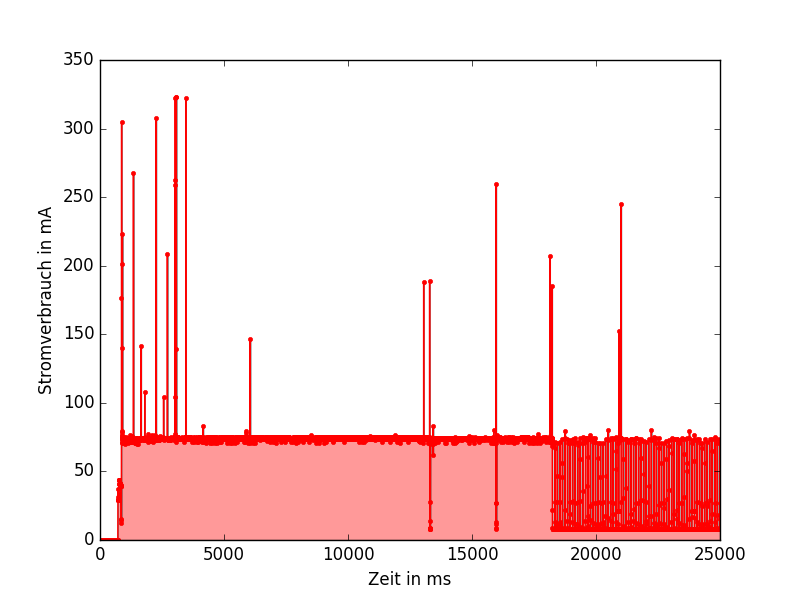
\includegraphics[width=\textwidth]{plots/radar5s.png}
  \caption{Stromverbrauchskurve einer Implementierung von \emph{RADAR}.}
  \label{fig:radar5s}
\end{figure}

Abbildung \ref{fig:radar5ssend} zeigt den Sendevorgang der \emph{RADAR-Implementierung}.
Auffällig ist, dass längerfristig empfangen wird, obwohl dies für den Versand des UDP-Pakets nicht notwendig ist.

\begin{figure}[h!]
  \centering
	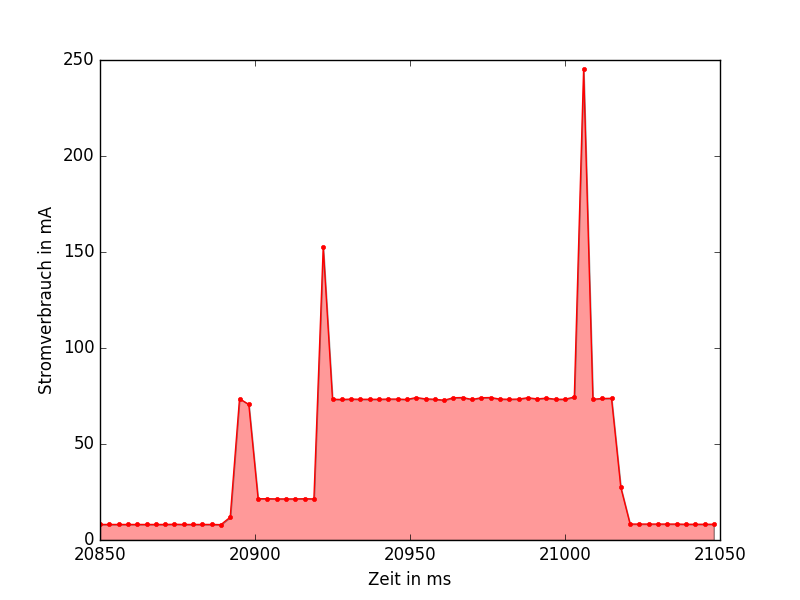
\includegraphics[width=\textwidth]{plots/radar5ssend.png}
  \caption{Stromverbrauchskurve eines Ortungsvorgangs mit RADAR.}
  \label{fig:radar5ssend}
\end{figure}

In Tabelle \ref{table:radarina} ist der durchschnittliche Verbrauch der \emph{RADAR}-Implementierung über eine Stunde gelistet.
Es wurde sowohl mit dem \emph{ESP8266} Feather, als auch mit dem einzelnen \emph{ESP-12F} gemessen, die mobile Einheit wurde jeweils erst circa eine Sekunde nach Beginn mit Strom versorgt.
Für den normalisierten Stromverbrauch wurde der Verbrauch im Ruhezustand subtrahiert. 
Dies beschränkt den Verbrauch auf den für die tatsächliche Funktion nötigen Anteil.

\begin{table}[h!]
	\centering
	\caption{Stromverbrauch mobiler Einheiten mit \emph{RADAR}-Implementierung}
	\label{table:radarina}
	\begin{tabular}{l|l|R{2.5cm}|R{2.5cm}}
		Hardware & Programm & $\varnothing$ Verbrauch in mA (normalisiert) & Laufzeit in Stunden\\
		\hline
		\emph{ESP8266} Feather & RADAR & 16,7 (8,6) & 83,8\\
		\emph{ESP-12F} & RADAR & 10,1 (8,8) & 138,6\\
	\end{tabular}
\end{table}

\subsubsection{Probe-Request-Lokalisierung}
\label{ch:phase2:sec:powerprobereq}
Abbildung \ref{fig:probereqfull} zeigt den Lastverlauf für eine mobile Einheit mit \emph{Probe-Request}-Implementierung und Abbildung \ref{fig:probereqv} zeigt den Lastverlauf für den Sendevorgang, der Verlauf für den \emph{ESP8266} Feather ist in rot und der Verlauf für das \emph{ESP-12F} Moduls ist in grün dargestellt.

Nachdem der \emph{ESP8266} aus dem \texttt{deep\_sleep} erwacht, beginnt eine circa 100 ms andauerne Startphase, danach sendet er die drei \emph{Probe Requests}.
Anschließend soll der \emph{ESP8266} wieder in den \texttt{deep\_sleep} versetzt werden, vorher empfängt er jedoch noch 100 ms.
Die restliche Zeit befindet sich der \emph{ESP8266} im Tiefschlaf. 
Bei dem \emph{ESP-12F} Modul ist der INA219 nicht in der Lage einen Stromvebrauch zu messen, er liegt unter 0,1 mA.

\begin{figure}[h!]
  \centering
	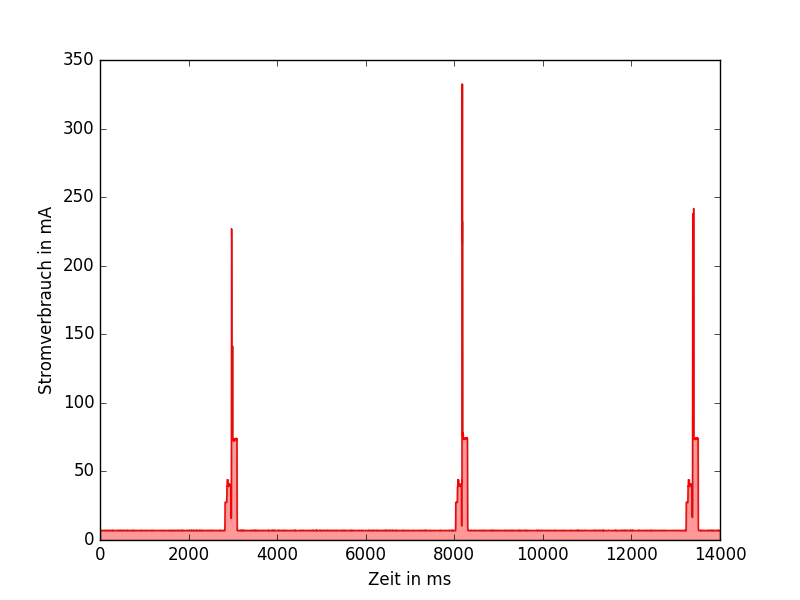
\includegraphics[width=\textwidth]{plots/probereqfull.png}
  \caption{Stromverbrauchskurve einer Implementierung mit \emph{Probe Requests}.}
  \label{fig:probereqfull}
\end{figure}

\begin{figure}[h!]
  \centering
	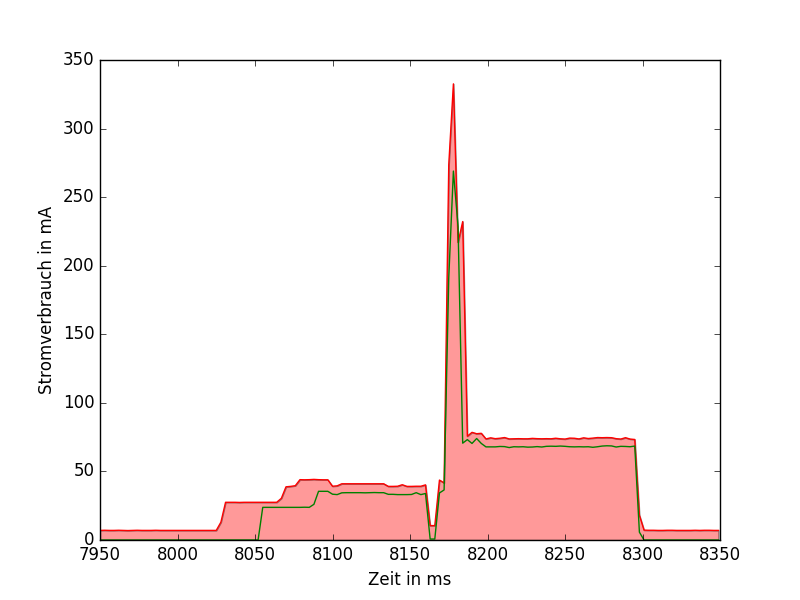
\includegraphics[width=\textwidth]{plots/probereqv.png}
  \caption{Stromverbrauchskurve eines Ortungsvorgangs mit \emph{Probe Requests}.}
  \label{fig:probereqv}
\end{figure}

Beim \emph{ESP8266} Feather misst er jedoch durchgehend einen Vebrauch von über 7 mA, daraus ergeben sich die Unterschiede in den Messungen, die in Tabelle \ref{table:probereqina} dargestellt werden.
Es wurde sowohl mit nur einem versendeten \emph{Probe Request}, als auch mit drei \emph{Probe Requests} getestet, die Unterschiede im Verbrauch liegen jedoch im Bereich der Messungenauigkeit.
Für den normalisierten Stromverbrauch wurde der Verbrauch im Ruhezustand subtrahiert. 
Dies beschränkt den Verbrauch auf den für die tatsächliche Funktion nötigen Anteil.

\begin{table}[h!]
	\centering
	\caption{Stromverbrauch mobiler Einheiten mit \emph{Probe-Request-Lokalisierung}}
	\label{table:probereqina}
	\begin{tabular}{l|p{5.3cm}|R{2.5cm}|R{2.2cm}}
		Hardware & Programm & $\varnothing$ Verbrauch in mA (normalisiert) & Laufzeit in Stunden\\
		\hline
		\emph{ESP8266} Feather & \emph{Probe-Request-Lokalisierung} drei Kanäle & 9,7 (2,7) & 144,0\\
		\emph{ESP-12F} & \emph{Probe-Request-Lokalisierung} drei Kanäle & 1,8 (1,8) & 777,8\\
		\emph{ESP8266} Feather & \emph{Probe-Request-Lokalisierung} ein Kanal & 9,7 (2,7) & 143,7\\
		\emph{ESP-12F} & \emph{Probe-Request-Lokalisierung} ein Kanal & 1,8 (1,8) & 769,2\\
	\end{tabular}
\end{table}

\subsection{Beschleunigungssensor}
\label{ch:Beschleunigungssensor}
Um den Stromverbrauch der \emph{Probe-Request}-basierten Lösung weiter zu senken wird in diesem Abschnitt die Einbindung eines Beschleunigungssensors, in Anlehnung an die kommerzielle Lösung von Ekahau \footnote{\url{https://www.airistaflow.com/}}, diskutiert. 

Im Tunnel Rastatt, in dem auch die Versuche stattfanden, arbeiten die Bauarbeiter in zwei Schichten zu je zwölf Stunden. 
Nach zehn Tagen Schicht hat ein Arbeiter fünf Tage frei, jeder Arbeiter arbeitet also genau ein Drittel der Gesamtzeit. 

Die mobile Einheit behält jedoch derzeit seinen Senderythmus bei, angesichts des hohen Stromverbrauchs beim Senden ist dies ineffizient.
Ein Beschleunigungssensor soll bestimmen, wann die mobile Einheit in Bewegung ist. 
Dadurch wird sie nicht mehr senden, wenn sie nicht getragen wird.

\subsubsection{LIS3DH}
Der \emph{LIS3DH} ist ein Drei-Achsen-Beschleunigungssensor von ST Microelectronics \cite{st2015lis}.
Er zeichnet sich durch einen \emph{ultra-low-power} Modus und einen Pin für externe Unterbrechung (\emph{Interrupt}) aus.
Der Beschleunigungssensor bietet ein $I^2C$ und ein \emph{SPI Interface} um ihn zu konfigurieren.
Der \emph{LIS3DH} benötigt bei einer Frequenz von einem Herz nur 2 \textmu A (0,002 mA).

Leider konnte bei einem Herz der \emph{Interrupt} durch Laufbewegungen nicht sicher ausgelöst werden, die Frequenz wurde deshalb auf zehn Herz erhöht.
Für eine Frequenz von zehn Herz im \emph{ultra-low-power} Modus listet das Datenblatt einen Verbrauch von 3 \textmu A.
Abbildung \ref{fig:lis3dh} zeigt eine Platine mit integriertem \emph{LIS3DH}.

\begin{figure}[h]
  \centering
	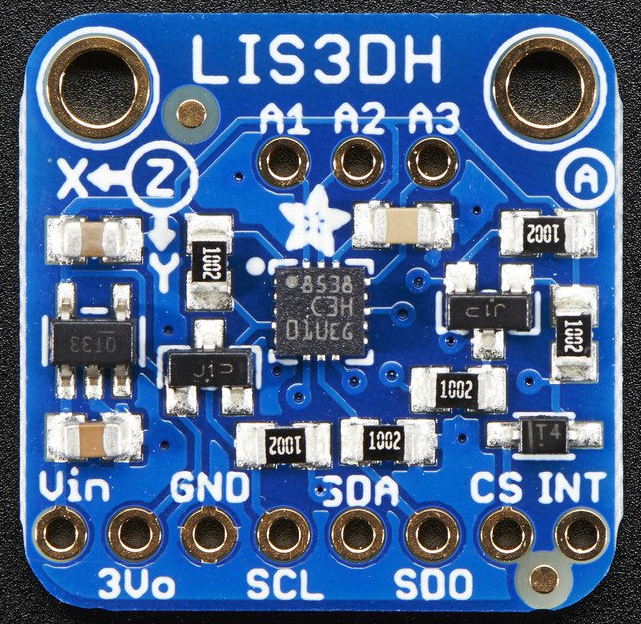
\includegraphics[width=0.5\textwidth]{images/lis3dhada.png}
  \caption{\emph{LIS3DH} integriert auf einer Platine für die Entwicklung. Bild von Adafruit Industries\protect \footnotemark.}
  \label{fig:lis3dh}
\end{figure}
\footnotetext{\url{https://www.adafruit.com/product/2809}}

\subsubsection{Abschaltautomatik}
\label{ch:Beschleunigungssensor:sec:Abschaltautomatik}
Der \emph{ESP8266} besitzt einen \emph{Enable Pin} (CH\_PD), ist dieser mit der Versorungsspannung verbunden werden die internen Spannungregler aktiviert und der \emph{ESP8266} mit Strom versorgt.
Die eigentliche Stromversorgung bezieht er dabei jedoch aus dem \emph{Vcc Pin}.
Der \emph{ESP8266} soll durch den \emph{LIS3DH} angeschaltet werden, der \emph{ESP8266} darf die Stromversorgung bei Bedarf trennen, sie kann danach wieder vom \emph{LIS3DH} wieder aktiviert werden. 

Um dieses Verhalten zu erreichen wird ein \emph{Latch} eingesetzt \cite{texas2003latch}.
Es handelt sich dabei um einen digitalen Schalter mit einem SET-Eingang (An), einem RESET-Eingang (Aus) und einem Ausgang.
Der Ausgang wird mit dem \emph{Enable Pin} verbunden, ist er aktiv, wird der \emph{ESP8266} aktiv.
Der SET-Eingang wird mit dem \emph{Interrupt Pin} des \emph{LIS3DH} verbunden, er kann damit den den Ausgang aktivieren.
Der RESET-Eingang wird mit dem \emph{ESP8266} verbunden. 
Es wurde \emph{Pin 16} ausgewählt, da dieser für das Aufwecken aus dem Tiefschlaf zuständig ist. 
Stattdessen soll er nun die Stromversorgung abschalten und durch die zuvor im \texttt{deep\_sleep} verbrachte Zeit das Sendeintervall abwarten.

Da das Aufwecken mit \emph{Pin 16} durch das Verbinden des Pins mit der Masse funktioniert, kann damit nicht direkt der RESET-Eingang des Latches betrieben werden.
Stattdessen wird das Ergebnis von \emph{Pin 16} mit der Versorgungsspannung über ein XOR-Gatter verschaltet und mit dem RESET-Eingang verbunden \cite{texas2014xor}.
Abbildung \ref{fig:schematics} zeigt das Schema der Verbindung von \emph{ESP8266} und \emph{LISD3H}.

\begin{figure}[h]
  \centering
	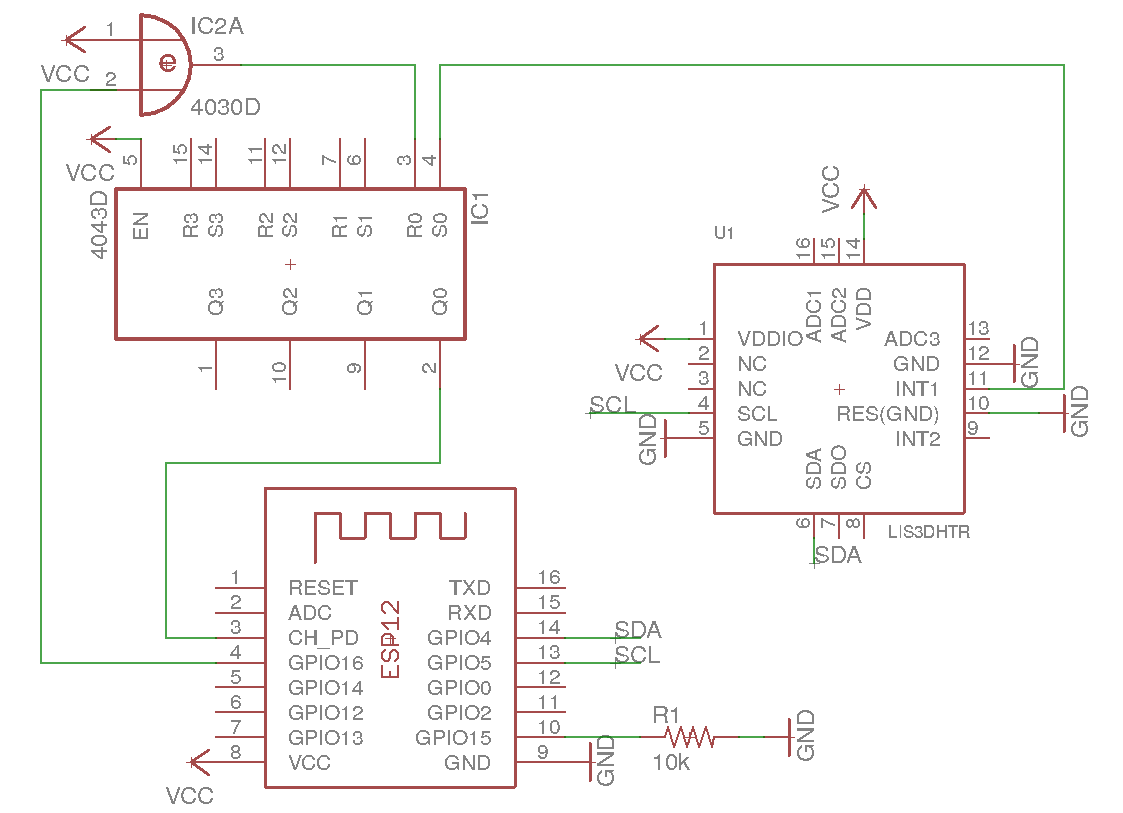
\includegraphics[width=\textwidth]{images/schematics.png}
  \caption{Schema der Verbindung von \emph{ESP8266} und \emph{LIS3DH}.}
  \label{fig:schematics}
\end{figure}

\subsubsection{Bewertung}
Der Verbrauch des Beschleunigungssensors ersetzt lediglich den Verbrauch des Mikrocontrollers, die anderen Komponenten bleiben davon unberührt.
Zu den 3 \textmu A Verbrauch addiert sich deshalb der Verbrauch des Spannungswandlers (55 \textmu A) und des Lithium-Polymer-Ladeschaltkreises (bis zu 100 \textmu A).
Hinzu kommen bis zu 1 \textmu A für das \emph{Latch} und 10 \textmu A für das XOR-Gatter.

Die Integration des Beschleunigungssensor kann also den Verbrauch des \emph{ESP8266} außerhalb der Arbeitszeiten durch einen Verbrauch von 14 \textmu A ersetzen, die bis zu 166 \textmu A Verbrauch der umliegenden Komponenten bleibt jedoch vorhanden.
Die Laufzeit für eine nicht bewegte mobilen Einheit mit \emph{ESP8266} beträgt dann mindestens $1400mAh / 0,18mA = 7777,77h$, dies entspricht ca. 324 Tagen.

Bei den vorherigen Prototypen, die eine \emph{Assoziation} erforderten, muss beachtet werden, dass sie nach dem erneuten Anschalten einen \emph{Scan}- und \emph{Join}-Vorgang ausführen.
Damit diese die Einsparung nicht überwiegen, sollte eine Abschaltung erst nach einigen Minuten der Inaktivität erfolgen.


